\section{Signal formation on resistive strips: the sharing kernel}\label{sec:kernel}
\sectionstate{ready}{\texttt{sps\_beam\_test\_26/analysis/sharing\_kernel}, \texttt{angled\_kernel}, \texttt{plane\_ratio/FINDINGS.md}; \texttt{cloud\_basics} \S27--34}
\intent{Measure, model-free and head-on in the beam, how a strip's charge reaches its neighbours: amplitude and delay
to $\pm1$ and $\pm2$, gain-invariant, rotation-invariant, attachment-proof. The physical requirement $c_2<c_1$.}

\tbw{Y: $c_2/c_1$ = 0.42--0.47 at three fields; $\pm1$ delay $\sim$49\,ns; gain-invariant to 1--3\,\% (run\_66);
survives a 25.6\textdegree{} rotation. X: $\pm2/\pm1\approx$ 0.15--0.20 on all five chambers, against 0.36--0.54 in Y.
det4 $D_{RC}$ = $2.2\times10^{-4}$ ($\pm$10\,\%) in the beam. $\tau$ and $c_2$ are bounds: the tail outlasts the 3.84\,\textmu s window.}
\analysis{X-width}{the X-width excess (cloud\_basics \S28--34) is unsolved: state it as a limitation or explain it}
\askStephan{Expected RC constant of the resistive strips through the insulator (sheet resistance, kapton thickness): does $D_{RC}$ match the design?}
\begin{figure}[t]
  \centering
  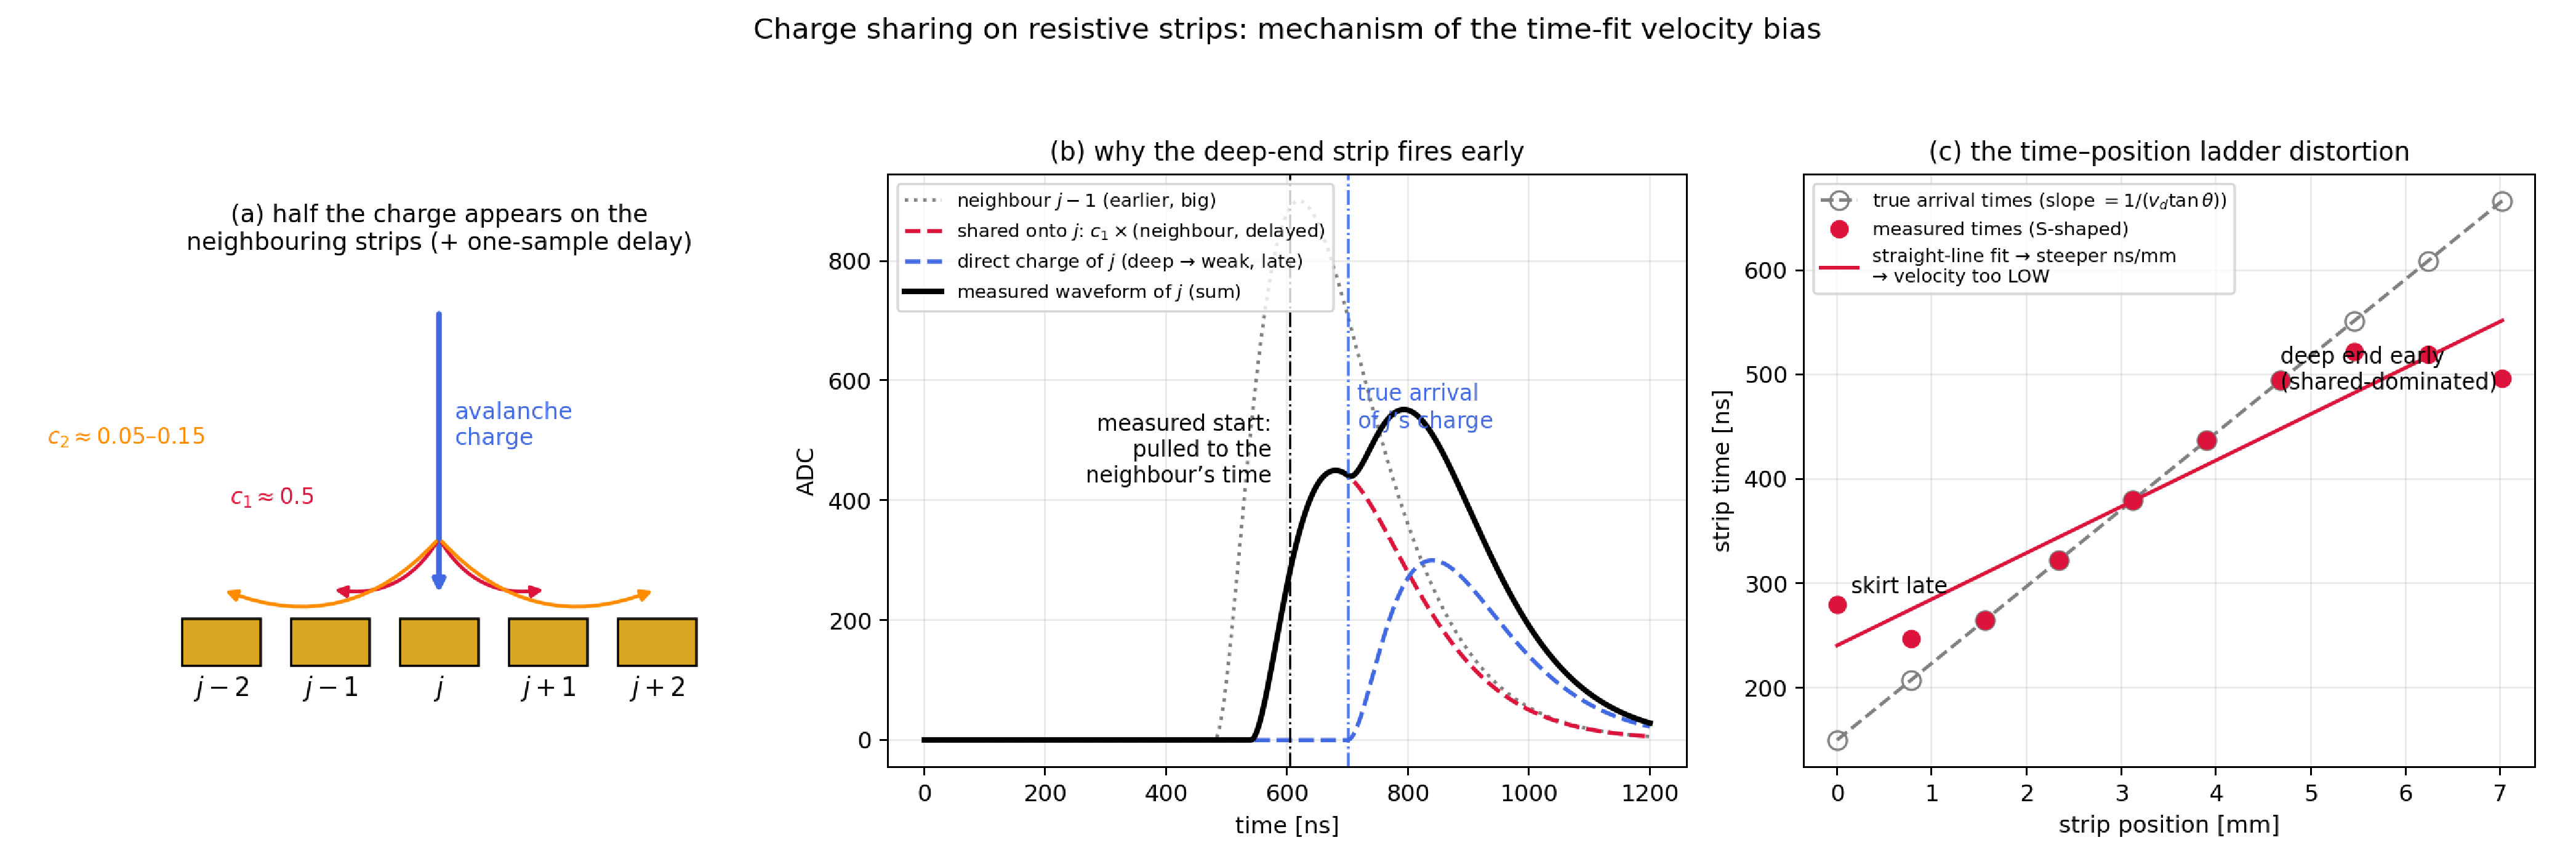
\includegraphics[width=0.7\linewidth]{sharing_cartoon}
  \caption{\tbw{How charge reaches the neighbouring strips.}}
  \label{fig:sharing_cartoon}
\end{figure}
\begin{figure}[t]
  \centering
  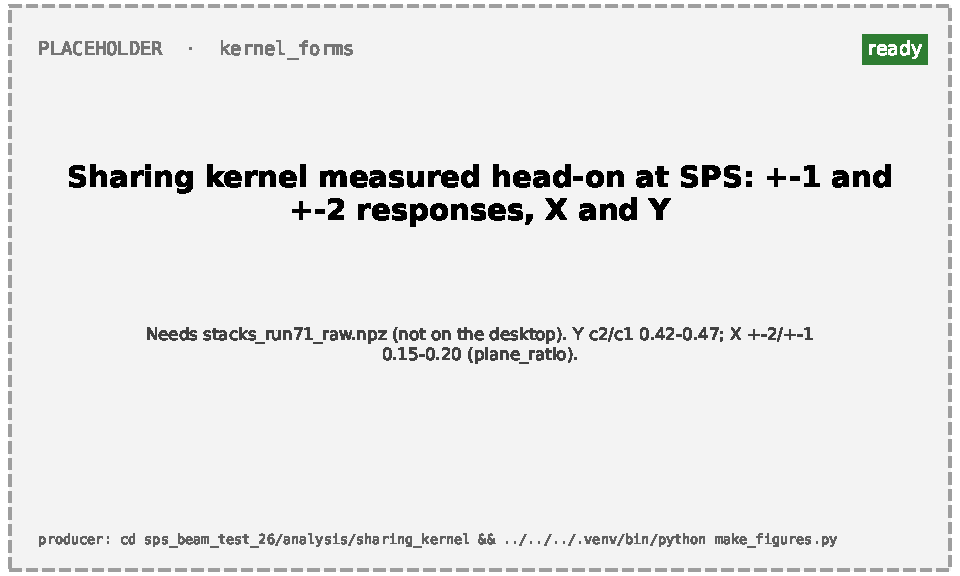
\includegraphics[width=0.9\linewidth]{kernel_forms}
  \caption{\tbw{Kernel forms measured head-on, X and Y.}}
  \label{fig:kernel_forms}
\end{figure}
\begin{figure}[t]
  \centering
  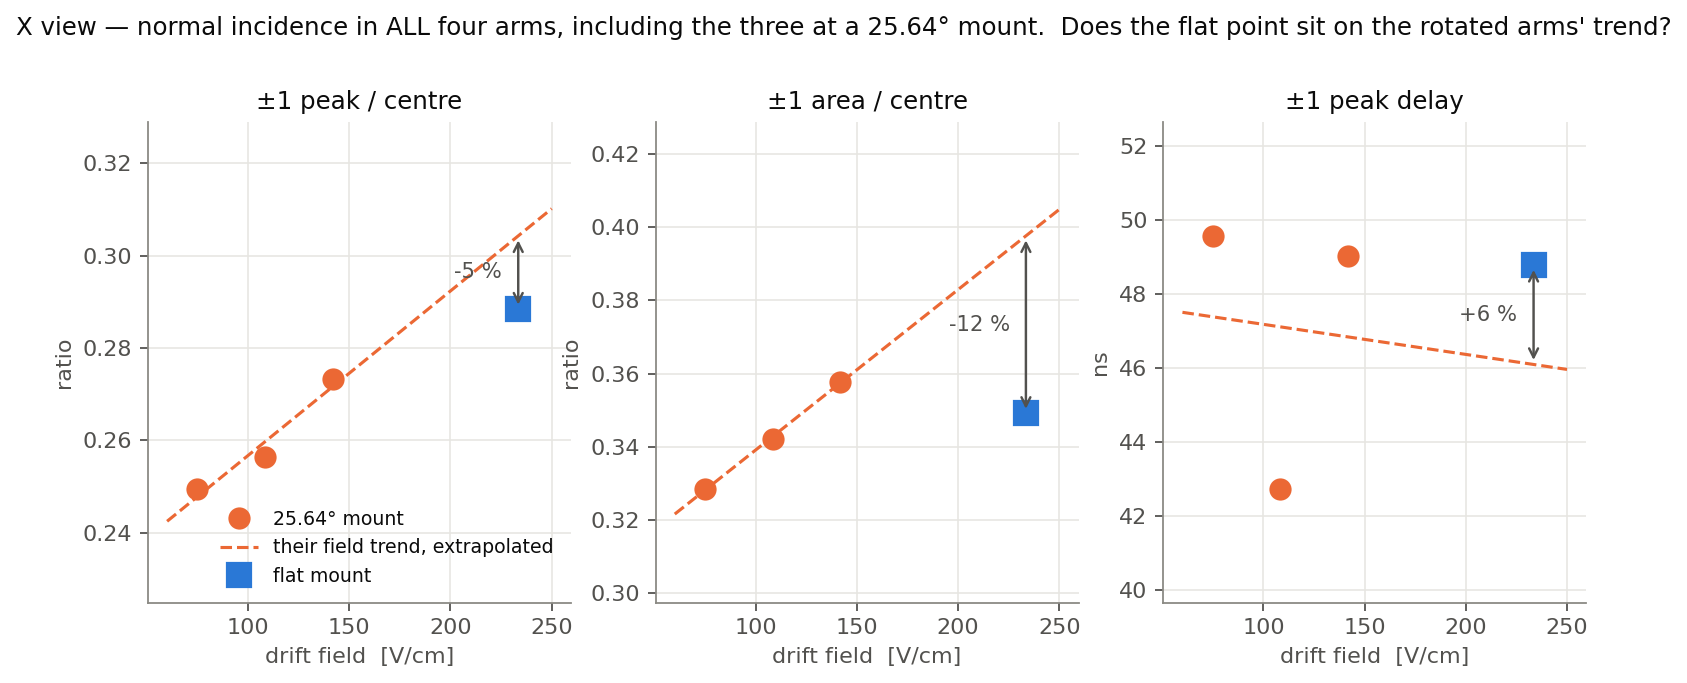
\includegraphics[width=0.7\linewidth]{angled_kernel}
  \caption{\tbw{The kernel at a 25.6 degree rotation.}}
  \label{fig:angled_kernel}
\end{figure}
